%%%%%%%%%%%%%%%%%%%%%%%%%%%%%%%%%%%%%%%%%%%%%%%%

\documentclass[12pt, a4paper]{report}
\usepackage[utf8]{inputenc}
\usepackage{amsmath}
\usepackage{amsfonts}
\usepackage{amssymb}
\usepackage{graphicx}
\usepackage{booktabs}
\usepackage[export]{adjustbox}
\usepackage[style=apa, backend=biber]{biblatex}
\DefineBibliographyStrings{english}{%
  bibliography = {References},
}

%%%%%%%%%%%%%%%%%%%%%%%%% ADD ANY ADDITIONAL PACKAGES BELOW
% Uncomment for blank lines between paragraphs rather than
% indents
\usepackage[parfill]{parskip}
\usepackage{pdfpages}

%%%%%%%%%%%%%%%%%%%%%%%%%%%%%%%%%%%%%%%%%%%%%%%%%%%%%%%%%%%%


%%%%%%%%%%%%

\addbibresource{refs.bib}

\usepackage[linktocpage=true]{hyperref}	% This creates hyperlinks and moves the contents links to the page number for clarity
% There are lots of options you can alter to what you want, see http://www.tug.org/applications/hyperref/manual.html
\usepackage[font=small,labelfont=bf]{caption}	% This ensures hyperlinks to figures link to the top of the figure not the caption. This line must come after the previous one (hyperref package).
\linespread{1.3}


\begin{document}
\pagenumbering{alph}	% This stops the title page being counted in the page numbering
\thispagestyle{empty}	% This stops a number being put at the bottom
\vspace*{1mm}	% The asterisk is needed because it's at the top of a page
% \includegraphics[width=0.8\textwidth, center]{./figures/UoP_Master_Logo_Linear_PMS.eps}
\vspace{10mm}

\begin{center}
% Put the full title  on the front page
\huge\textbf{\textsf{Fine-Tuning SOTA sEMG Silent Speech Models for Multiple Downstream Tasks}}\\
\vspace{15mm}
% The student handbook states you need your full name on the front page
\large \textbf{Tada Makepeace}\\


\vspace{10mm}
\normalsize School of Computing \\ Final Year Research Project \\

\vspace{20mm}
%
\today	% This prints todays date, eg. ``January 1, 2012``.
% Make sure all of the above fits on the front page, otherwise you will have to change the spacings, eg. to accomodate a long title
\end{center}
\newpage
\pagenumbering{roman}	% This sets page numbers to be Roman numerals for the preliminaries
\phantomsection	% This makes the abstract's bookmark link to the top of the page instead of the title line.
\addcontentsline{toc}{chapter}{Abstract}	% Gives the Abstract a contents entry
\chapter*{Abstract}	% The asterisk stops a chapter number being assigned

No more than 300 words summarizing this dissertation.

\newpage
\renewcommand{\contentsname}{Table of Contents}	% Changes the contents title from 'Contents' to 'Table of Contents' just because it looks better.
\pdfbookmark{Table of Contents}{contents}	% Adds a bookmark 'Table of Contents' in the PDF and labelled 'contents' for the hyperref package.
\tableofcontents

\newpage
\pdfbookmark{List of Tables}{tables}	% Adds a bookmark 'List of Tables' in the PDF and labelled 'tables' for the hyperref package.
\listoftables

\newpage
\pdfbookmark{List of Figures}{figures}	% Adds a bookmark 'List of Figures' in the PDF and labelled 'figures' for the hyperref package.
\listoffigures

% The commands for the preliminary sections below serve the same purposes as for the abstract section above, You can add or remove sections as you see fit.
% Here might also be a good place to put a dedication if you want.
%\newpage
%To...

\newpage

\phantomsection
\addcontentsline{toc}{chapter}{Acknowledgements}
\chapter*{Acknowledgements}
Thanks.
\newpage


\pagenumbering{arabic}	% Begins normal page numbering for the body of the report.


%%%%%%%%%%%%%%%%% INCLUDE YOUR CHAPTERS BELOW
% for each chapter, create a new .tex file (e.g. litreview.tex) and then use \include to include them in your output. Use a descriptive name, not their number (as these can change!).
% If you move the order around, all the cross references remain, sensibly renumbered.
% yay!
\chapter{Introduction} \label{chap:intro}
A gentle reminder not to get this chapter perfect until the dissertation is nearing its completion\ldots

\section{A section}

\subsection{A sub-section}

\subsubsection{A sub-sub-section}



\section{Citations}

When it comes to referencing, if we want to assert a fact and then provide its reference use \verb!\parencite!. For example -- one should adapt feedback to learner personality \parencite{dennis2016adapting}.

Or if you want to talk about the research directly, use \verb!\textcite!: \textcite{dennis2016adapting} did a PhD in adapting feedback to learner personality. 

If you want to cite two sources at the same time, you can separate the keys with commas \parencite{dennis2016adapting,cle12}.

\section{Figures}

\begin{figure}
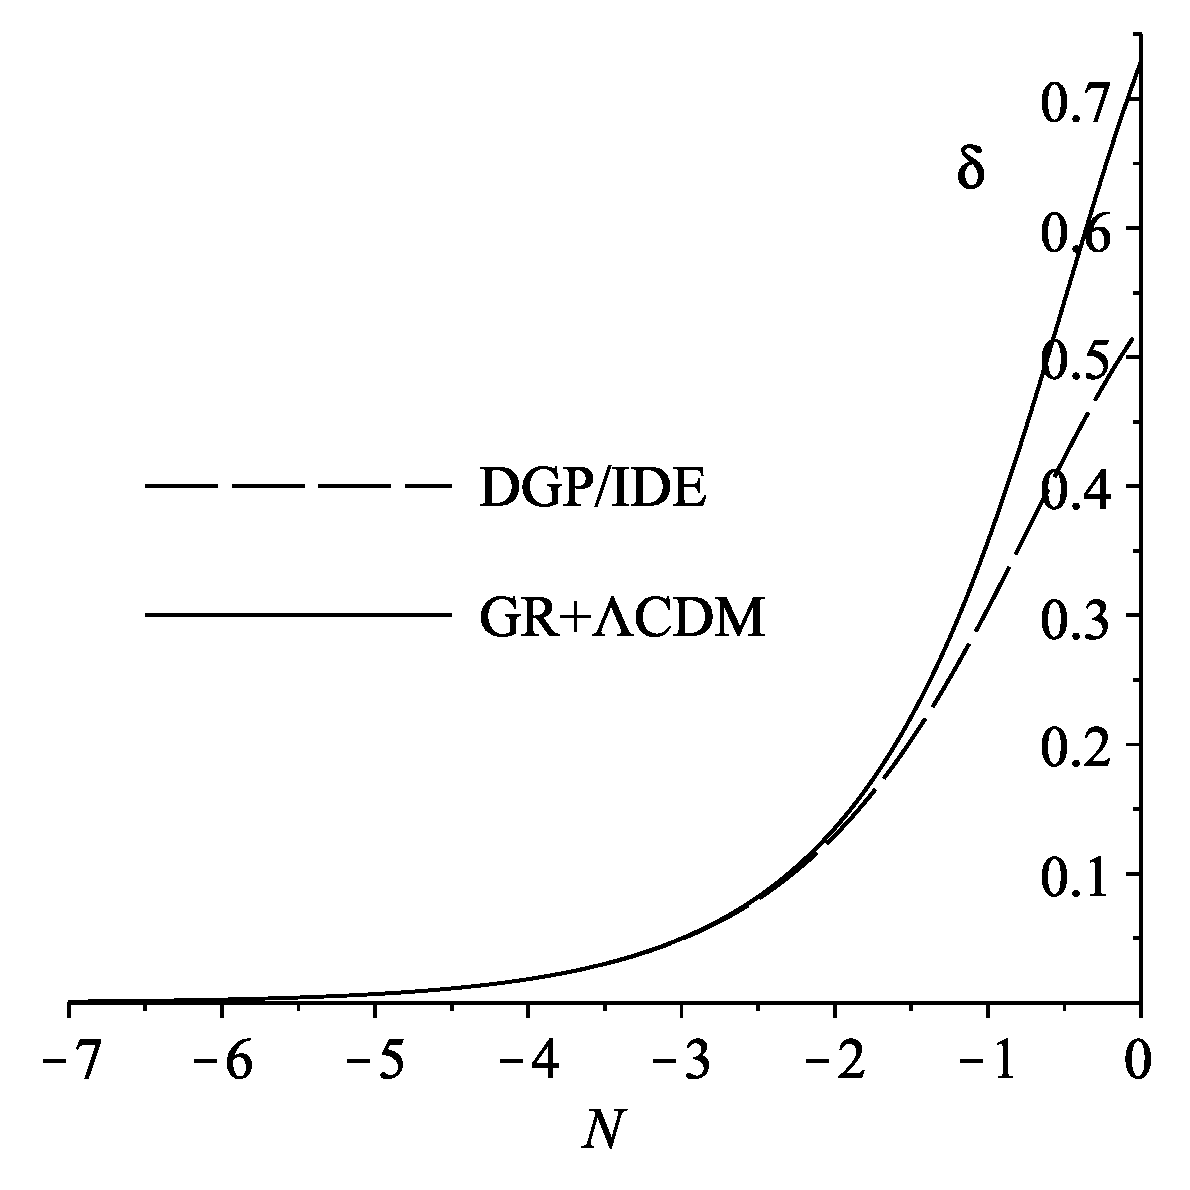
\includegraphics[width=0.49\columnwidth]{figures/dgpdeltas.eps}
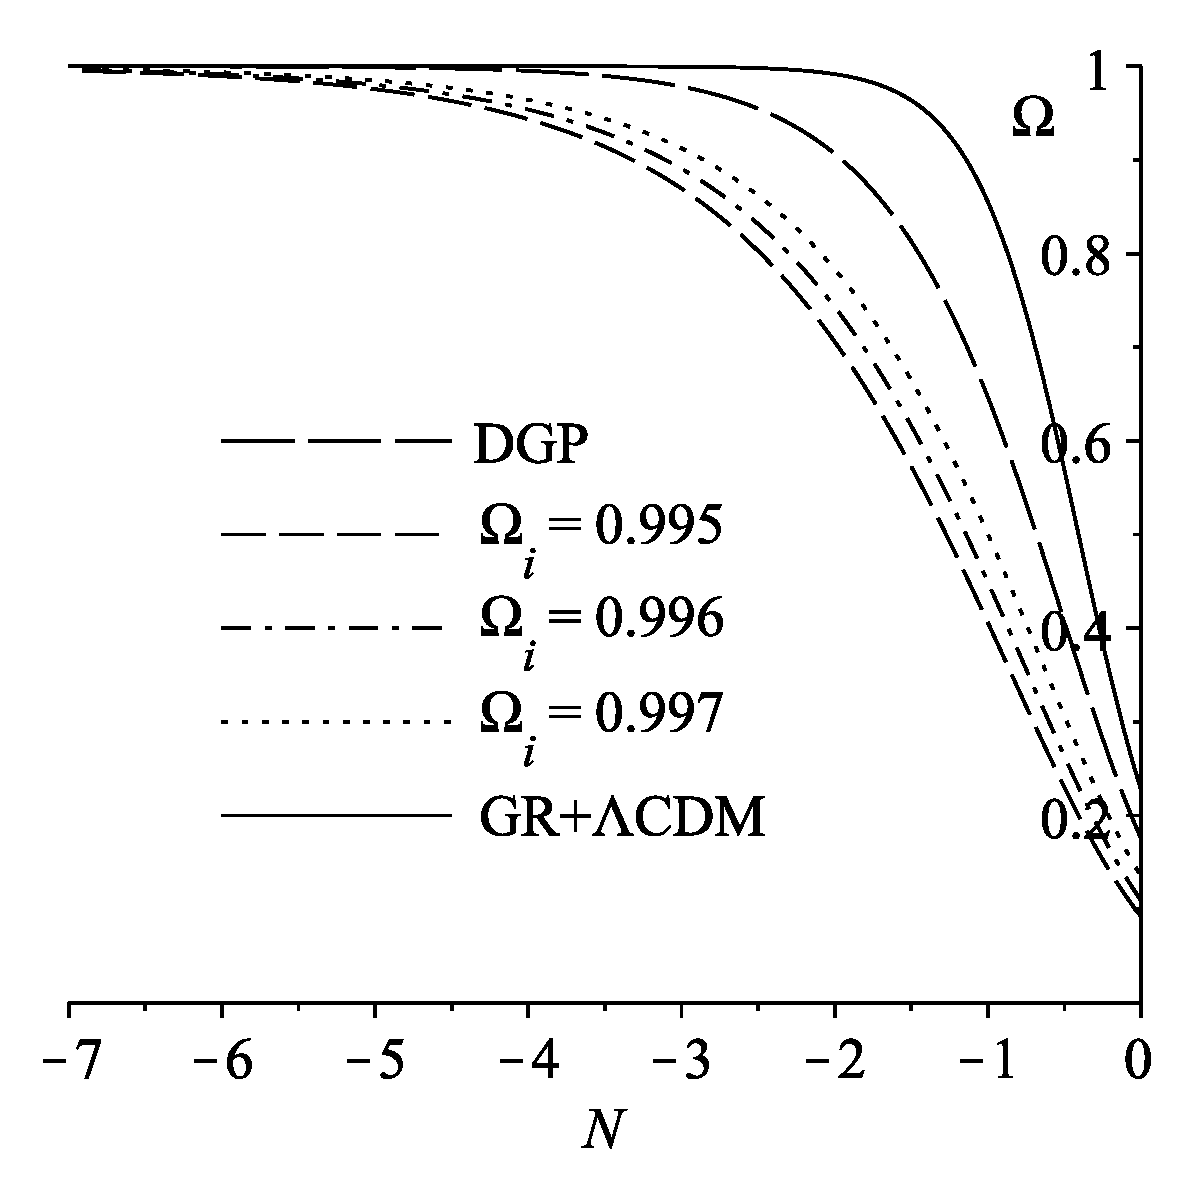
\includegraphics[width=0.49\columnwidth]{figures/dgpomegas.eps}
% For long captions include a short version for the List of Figures/Tables sections in square brackets as below.
\caption[Evolutions of $\delta$ and $\Omega$ for DGP]{Evolution of the density perturbation (left) and the density parameters (right) for the matched DGP/IDE models, each with a different $\Omega_i$,
and a GR+$\Lambda$CDM model.
\label{fig:matched}}
\end{figure}

Don't the graphs in \autoref{fig:matched} look scary? Don't worry, this is because I adapted this template from ICJS. Remember - if you are including screenshots or other raster graphics (i.e. PNG, JPEG) you should ensure that they are at least 300dpi. This will take effort on your part - most people's screens are at 72dpi.   

Vector is better (EPS or PDF) if you can manage it. If you are exporting graphs from Microsoft Excel for example, place the chart in its own sheet and print it to PDF. Then, using Acrobat or similar, crop the whitespace off the PDF. This is the most reliable way I have found to include vector graphics from Microsoft Office.







% To include math symbols in things with hyperlinks you need to specify an alternative plain text version for the bookmark using \texorpdfstring as below:
\section{A section with math symbols, eg. \texorpdfstring{$\Lambda$}{Lambda}CDM}
test test test test test test test test test test test test test test test test test test test test test test test test test test test test test test test test test test test test test test test test
test test test test test test test test test test test test test test test test test test test test test test test test test test test test test test test test test test test test test test test test
test test test test test test test test test test test test test test test test test test test test test test test test test test test test test test test test test test test test test test test test
test test test test test test test test test test test test test test test test test test test test test test test test test test test test test test test test test test test test test test test test


\chapter{Research Questions} \label{chap:research-questions}

\section{List of Research Questions}

\begin{itemize}
    \item \textit{Can fine tuning an ASR model on transduction predictions
    improve performance on multiple downstream tasks?} \\
    Measurable: WER of final system compared to SOTA for text classification \\
    Measurable: WER of final system compared to SOTA for speech synthesis
\end{itemize}
\chapter{Literature Review} \label{chap:lit-review}

\section{Proposed Directions for Research}

\subsection{Data Augmentation}

It might be possible to use GANs (Generative Adversarial Networks) or
VAEs (Variational Auto Encoders) to create a model which can generate
more data samples.

\subsection{Improving Existing Model}

Use RL-Learning to find a model which can outperform the original model
(problem is small dataset size which means that the benfits of using RL
to create a model might not be as applicable to this problem).

Use CapsNet on top of the CNNs to improve the generalisability of the
detected EEG features (there are papers which show that these are
feasible).
\chapter{Approaches} \label{chap:approaches}

This chapter will describe the main dataset used for this research, why it was chosen,
the main EMG signals of interest from the dataset, methods of feature selection and
visualisation and the machine learning approaches used to transcribe the EMG data
into a text transcription.

\section{Dataset}

\subsection{Dataset Selection and Justification}

The dataset which is used throughout this research project is the open-source
surface electromyography silent speech (sEMG silent speech) dataset released
by David Gaddy along with his paper, Digital Voicing of Silent Speech
(\cite{gaddy2020digital}).
The paper describes a novel method of transcribing aligned silent speech data
directly into speech features along with the largest open-source sEMG silent
speech dataset.

This dataset was chosen for this research as it is the largest, high quality open
source sEMG silent speech dataset.

\subsection{Feature Selection}

For this research there were two primary ways of selecting features. The first method
was to use the same feature processing methods described in the original
(\cite{gaddy2020digital}) paper. The second method was to use a convolutional
neural network (CNN) architecture to automatically learn features from the
dataset, in an end-to-end manner.

\section{Models}

\subsection{DeepSpeech2 Model}

The DeepSpeech2 model was the initial automatic speech recognition (ASR) machine
learning model which was considered for experimentation as it is relatively simple to
implement and is known to have good performance, even on smaller datasets, achieving
a 3.10 WER on the WSJ eval'92 dataset
(\cite{DS2_original}).

\section{Baseline ASR Testing}

To get a realistic baseline for the possible performance of the silent
speech models, standard audio based ASR models were trained on different
slices of the Digital Voicing datasets audio and text transcriptions only.
The intuition for this was that an ASR model trained on the audio and text
transcriptions should in theory perform better than on the purely vocalised
EMG data or final silent EMG data and their respective text transcriptions.
The results of the baseline ASR models is provided below.

\subsection{Datasets}

Three main datasets were chosen for the baseline ASR tests. The first dataset
was the LJSpeech dataset
(\cite{ljspeech17})
which is an open-source dataset primarily used in
speech synthesis and also speech recognition. The remaining two datasets
are comprised of the audio and text transcriptions of vocalised
utterances from the Digital Voicing dataset release (\cite{gaddy2020digital}).
The first dataset from this data comes from utterances from the closed
vocabulary set of recordings during the vocalised condition from the dataset.
The second dataset from this data comes from
all of the audio and text transcriptions during the vocalised condition across
the entire dataset. The three datasets are referred to as
\textit{ASR-LJSpeech}, \textit{ASR-SilentSpeechVocal-Closed} and
\textit{ASR-SilentSpeechVocal-Full},
respectively.

The \textit{ASR-LJSpeech dataset} was chosen as it is a standard open-source dataset
used for speech related machine learning tasks. It also has similar, but greater
quantity of important properties than the \textit{ASR-SilentSpeechVocal-Full} dataset.
These include the vocabulary size,
average length of recordings and duration of the entire dataset. This intuitively
means that the DeepSpeech2 ASR model trained on the \textit{ASR-LJSpeech dataset} should
have a lower WER rate, so better performance, than trained on
the \textit{ASR-SilentSpeechVocal-Full dataset}.
Whereas the \textit{ASR-SilentSpeechVocal-Closed} dataset was chosen because it has
a far lower duration and vocabulary size than the \textit{ASR-SilentSpeechVocal-Full}
dataset which makes it a lot faster to experiment with as the training time is
lower.

\subsection{Implementation}

\subsection{Results}

The following results table shows the word-error rate for each dataset
which the DeepSpeech2 model was trained on. Each dataset used a slightly
different vocabulary. The vocabulary for each dataset
is the list of valid characters
of the text transcriptions which the model considers, any other characters
are encoded as \textless UNK\textgreater. A different vocabulary was chosen for the
ASR-SilentSpeechVocal-Closed dataset because it contains far more numbers
than the other datasets and including numbers in it's vocabulary means
that the transcriptions would be useful, rather than filled with the
unknown placeholder value.

% ALL OF THESE EXPERIMENTS NEED TO BE RE-RUN AT SOME POINT!

{\small\begin{center}
\captionof{table}{DeepSpeech2 Audio ASR Baseline Results}
\begin{tabular} { | l | c | c | }
\hline
Dataset & Encoding Vocabulary & WER \\
\hline
ASR-LJSpeech                 & " abcdefghijklmnopqrstuvwxyz-" & 0.55 \\
ASR-SilentSpeechVocal-Closed & " abcdefghijklmnopqrstuvwxyz0123456789-" & 0.33 \\
ASR-SilentSpeechVocal-Full   & " abcdefghijklmnopqrstuvwxyz-" & 0.45 \\
\hline
\end{tabular}
\end{center}}

%%%%%%%%%%%%%%% APPENDICES
\appendix

\chapter{Project Initiation Document}

\includepdf[pages=-]{./appendicies/PID_up904749.pdf}

% Ethics Review (Pre-FEC Signature)

\chapter{Ethics Review}

\includepdf[pages=-]{./appendicies/Ethics_Review.pdf}

%%%%%%%%%%%%%% REFERENCES SECTION
\newpage
\phantomsection
\addcontentsline{toc}{chapter}{References}
% In order to try and get a consistent format I copy and paste the INSPIRE bibtex code into my bibtex file.
\printbibliography



\end{document}